\section{A Series of Tubes - A Tool for Pipe Design}

As mentioned, pipe design is not trivial.  Independent pipes cannot intersect lest their contents be unintentionally mixed.  Pipes' bending energy needs to be minimized to allow for easy insertion of media post-print.  Pipes in general need to avoid the surface of objects to prevent fluid leakage when printed by hobbyist-grade machines.  Finally, for designing pipes that follow a user-specified path, we must ensure certain characteristics of that path (e.g., that the path is connected).

To allow makers to design novel objects with pipe-powered interfaces, we created a tool for use on arbitrary 3D models.  This tool allows designers to select exterior connection points of their pipes (see Figure \ref{fig:tool-process-interior}) or to import vector art describing the pipes' interior paths (see Figure \ref{fig:tool-process-exterior}).  Once the maker's selections are made, we create a complete routing using either the exterior connection point method (A*, physical simulation) or the interior path method (graph edge creation, Euler tour generation).  We thicken our routing to create pipes. \valkyrie{We also apply templates where appropriate (e.g., 3D cross-overs for tubes that intersect in the plane).}  The resultant pipes are subtracted from the original mesh, which can then be 3D printed.

Our tool is implemented as a part of Meshmixer, a consumer 3D mesh editing tool, in C++ \cite{Schmidt-meshmixer}.

\subsection{Exterior Connection Points}

Designing objects which, for example, are touch sensitive in particular areas or need to integrate with existing electronics, requires precise location and sizing of pipe endpoints.  The interior of these pipes should have as large a bending radius as possible so that post-print insertion of solid or viscous media (like wire or paint) is easier.

To create pipes in which the location and shape of exterior connection points matters, we first allow makers to select the connection points on the mesh's surface. Our tool then creates an initial shortest-path routing using A* to estimate the routed distance between points.  This routing is used to create a rod; we run physics-based simulation steps on the rod to minimize its bending energy (and thereby minimize the bend radius of the tubes).

\begin{figure}[h!]
\centering
    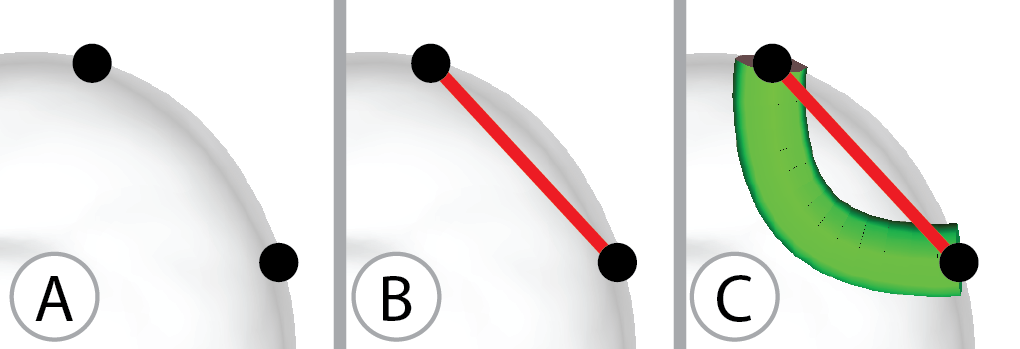
\includegraphics[width=3.4in]{figures/exterior.png}
\caption{An example mesh with exterior connection points selected.  The smoothed A* routing is drawn in {\color{red}red}, and in {\color{tovi}green} is our physically-based rod after simulation. \valkyrie{make a figure that is less... tall}}
\label{fig:tool-process-exterior}
\end{figure}

\subsubsection{Routing and Physical Simulation}

Our basic first-pass routing algorithm uses the A* routing algorithm \cite{Hart-Astar}.  This algorithm keeps a priority queue of points to check for routing based on a cost function; for each point it tags the distance from the start (e.g., startPoint = 0, startNeighbors=1, ...).  Once the end point is reached, we backtrack through the tagged points, always moving towards a lower-valued point.  The path cost in our implementation is based only on shortest distance between the starting and ending points, without weighting for distance from the surface, however the routed path is forced to stay inside the mesh's boundaries.  We route on the voxelized 3D grid of the mesh, and we use a resolution of 128x128x128 voxels. 

Note that pipes, once cut, become ``outside the mesh''.  This means that pipes cut in sequence cannot intersect each other.  However, we do not currently track previously-cut pipes for global optimization: we simply greedily select the best routing per pair of points (i.e., per pipe).

Given our initial routing, we create a rod of the same length.  To allow for easiest insertion of media post-print, our physical simulation step minimizes the bend radius of the generated rod.  In order to force our simulated rod away from the surface of the mesh, we create ``wind'' pushing inward from the exterior of the mesh.  This wind keeps the resulting pipe away from the surface. \valkyrie{Ryan: How does it actually work?}

\subsubsection{Pipes with Multiple Endpoints}
For the creation of pipes with multiple endpoints, for example the star topologies in Figure \ref{fig:toys} or tree topologies, makers can select interior faces of existing pipes as endpoints, and thereby create pipe networks by hand.  We do not currently offer any pipe network manipulation tools.

\valkyrie{To allow designers to create pipes with multiple endpoints (like the star topologies in Figure \ref{fig:toys}), we create 0-size mesh points in the center of the object, to which we attach one end of every pipe?}

\subsubsection{Pipes with Non-Round Endpoints}
\valkyrie{this section can probably be scrapped, along with Figure \ref{fig:meshmixer-endpoint}.}
Although start and end radius of pipes is configurable, our tool does not explicitly allow makers to design the \emph{shape} of their pipes' endpoints.  However, the larger Meshmixer package does allow brushing arbitrary shapes onto the surface and extruding them inward, as in Figure \ref{fig:meshmixer-endpoint}.  This technique can be used to create specially-shaped touch pads or to recess the footprint of an electronic component for it to sit flush with the object's surface.

\subsubsection{Semi-Closed and Fully Enclosed Pipes}
Users can select via a checkbox if they wish to cap one end, the other end, or both ends of their pipe.  The software simply creates an offset from the surface in these cases, so that material remains between the pipe and the surface after mesh modification.

\begin{figure}[h!]
\centering
    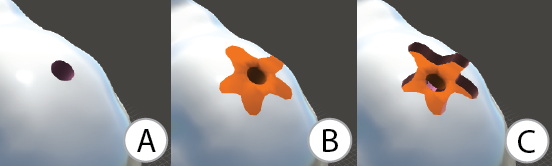
\includegraphics[width=3.4in]{figures/meshmixer-endpoint.png}
\caption{After creating a tube, a maker can select a surface shape using a brush (a).  She can then extrude her selection inward (b).}
\label{fig:meshmixer-endpoint}
\end{figure}

\subsection{Designing Interior Paths}

Neon signs, as in Figure \ref{fig:tool-process-interior}(d), require a single long path that passes through many desired edges: for example, in our UIST sign, the path must pass through all the edges that comprise the word ``UIST''.  To allow makers to create novel neon signs, as well as similar objects that require design of the pipe's interior path (for example the maze in Figure \ref{fig:maze}), we built a tool which leverages graph theory to generate this single long path.

A maker can import a vector graphics file (such as SVG) describing the path she desires for her pipes.  We create a graph based on this input data, then add edges to make it connected and semi-Eulerian.  We create an Euler tour on the modified graph, and thicken the path to create pipes.  \valkyrie{3D templates are used to resolve tube crossings in the plane.}  We cut these pipes from a generated block mesh large enough to hold them.

\begin{figure}[h!]
\centering
    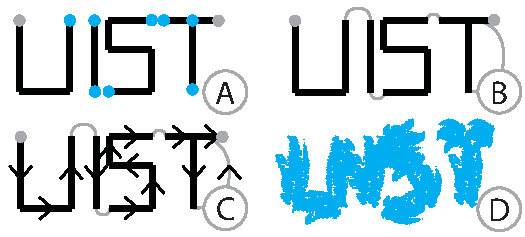
\includegraphics[width=3.4in]{figures/interior.pdf}
\caption{An input vector graphics file with the points which cannot be tubed as drawn highlighted in {\color{blue}blue} and the start and end points highlighted in {\color{gray}gray} (a).  The connected graph created by our software (b) and the resulting Euler circuit (c) permit creation of a novel neon sign (d). \valkyrie{for this sign, embed it in a fun hawaiian block}}
\label{fig:tool-process-interior}
\end{figure}

\subsubsection{Routing}
\tovi{Still too long....}
In graph theory, a semi-Eulerian graph is one which has exactly two edges of odd degree.  This kind of graph supports an Euler tour: a path that touches every edge exactly once, beginning and ending at the two nodes of odd degree (in this case, the user-selected start and end nodes).  To allow for a single path through a pipe for post-print media insertion, we need to find a semi-Eulerian graph for which a user's input graphics are a subset, and subsequently find an Euler tour on that graph.

The interior path routing problem is a version of the Chinese Postman Problem\footnote{The CPP is also known as the route inspection problem: \url{http://en.wikipedia.org/wiki/Route_inspection_problem}}, in which we wish to traverse all edges of the graph described in the user's input with a single Euler circuit, much as a postman needs to walk along every road at least once to deliver mail.  We call our relaxation the Spiderman Postman Problem: we allow the creation of non-existing paths (i.e., the postman may traverse buildings in addition to roads).  If input path components are disconnected, we must create edges that connect them; additionally we can create new edges connecting odd-degree vertices rather than simply retracing existing edges.  In the final artifact, all created edges will be blocked out by dark material so the inserted medium is not visible (see Figure \ref{fig:tool-process-interior}).  We offer a short algorithm here, with a more mathematically precise definition and associated proof in the appendix.

We need a graph which is semi-Eulerian (i.e., the inserted media can enter at one point, traverse every edge exactly once, and exit at a different point).  In order to create a semi-Eulerian graph, we first add a temporary edge to the start and end points.  This is removed after the graph is made fully Eulerian.

In order to connect disconnected subgraphs in the input, each disconnected subgraph's vertices and edges are contracted to a single vertex.  Each of these subgraph-vertices has no outgoing edges, as the expanded subgraphs are disconnected.  We then add one edge from each subgraph-vertex to each other subgraph-vertex, whose weight is the minimum distance between any two vertices in the expanded subgraphs (where distance is Euclidean distance).  We greedily select the smallest weight edges until all subgraphs are joined into a single graph.  We re-expand the subgraphs.

In order to make our graph Eulerian, we consider all vertices of odd degree in the connected graph and make a clique of edges once more based on distance.  We again greedily select edges between the odd nodes until no odd nodes remain.  Finally, we remove our temporary edge, which changes the graph from Eulerian to semi-Eulerian.  This graph is a connected, semi-Eulerian graph which contains all edges in the input SVG (see Appendix).

We believe that a lower total weight matching is possible by connecting components and ensuring edge degree evenness together in a global process, as well as by using minimum-weight matching rather than greedy selection, however this optimization is not crucial for our purposes.

Once we have a semi-Eulerian graph, we need to create an Euler tour.  We use a weighted modification of Fleury's algorithm for finding Euler tours\footnote{\url{http://en.wikipedia.org/wiki/Eulerian_path\#Fleury.27s_algorithm}} for this.  In the classic algorithm, each selected edge is removed to create a reduced graph.  To select the next edge while at a node, the algorithm randomly chooses from all incident non-bridge edges (where a bridge edge would create disconnected non-trivial subgraphs if it were removed).  This ensures that every edge is both reachable and traversed.  In our modification, instead of randomly selecting from non-bridge paths at each node, we select the non-bridge edge which turns the least from the most recent path (i.e., we prefer to pass straight through a node, if possible).  This minimizes turns in the final artifact, which eases support material removal and assembly.

\begin{figure}[h!]
\centering
    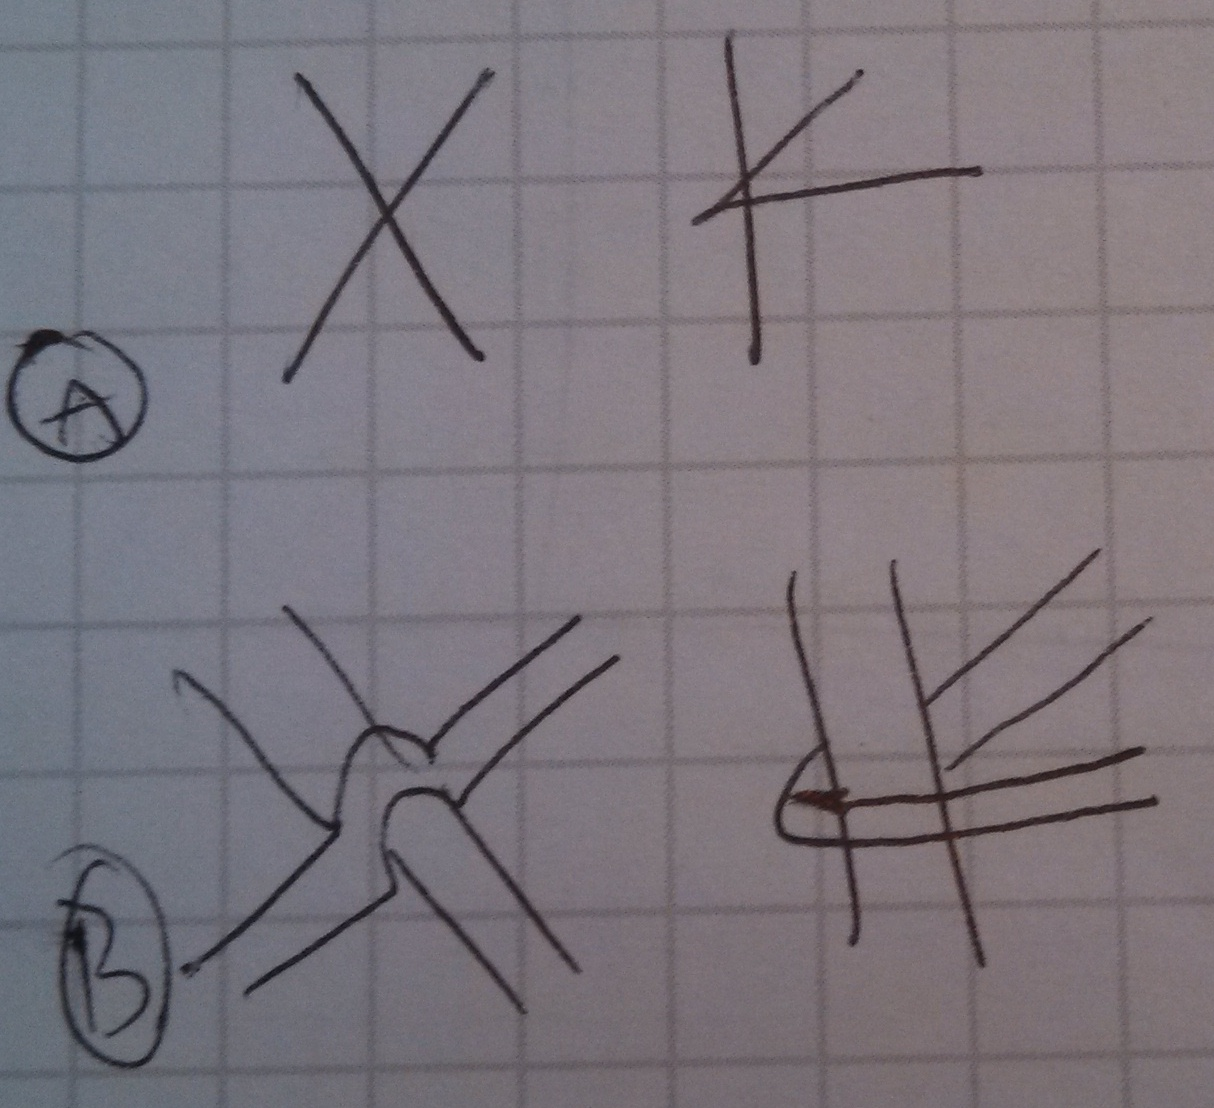
\includegraphics[width=3.4in]{figures/placeholder/templates.jpg}
\caption{\valkyrie{When edges intersect in the plane (a), we match them to the nearest of our several intersection templates (b) to create 3D paths that do not interfere with each other.}}
\label{fig:templates}
\end{figure}

\subsubsection{Edges that Intersect in the Plane}
We do not currently redirect edges that intersect in the plane.  Because we have a 3-dimensional canvas in which to work, it would be possible to push overlapping paths into the third dimension.  However, we leave this to future work: for our specific applications so far, it has been unnecessary.

\valkyrie{Once we have a tour, we must resolve tubes that intersect in the plane.  Because we have a 3-dimensional canvas in which to work, we can push overlapping paths into the third dimension.

To detect intersecting edges, we \valkyrie{I'm not sure what we do.}.  We also consider edges at nodes with degree $>2$, as these edges are considered to cross.  When intersections have been detected, we match one of several templates to the affected edges (see Figure \ref{fig:templates}) using a nearest neighbors technique.  Our templates are parameterized, so the templates can be modified to accommodate precise intersection characteristics.}

\subsection{Mesh Modification}

Given either our rod-based or image-based routing, we create cylinders which use the routings as a sweep path.  At each point in the routing, we create a cylinder tall enough to reach to the next point which is oriented along the line segment connecting its origin point to its destination point.  This cylinder's radius is set by the user.  For the rod-based routing, we allow independent start and end radii; in this case, the cylinder's radius is $\frac{k}{n}*\frac{r_1}{r_2}$, where $k$ is the point's index in the routing, $n$ is the total number of points in the routing, $r_1$ is the starting radius, and $r_2$ is the ending radius.

All cylinders generated are joined into a large rod.  This rod is voxelized, along with the original mesh.  These two voxel grids are subtracted, and the result is re-meshed and smoothed.  When a user desires to cap the ends of her pipes, we create a sphere of the same radius as each endpoint whose center is the same as the endpoint.  We intersect this sphere with the original mesh, then intersect this partial-sphere mesh with a shell of the original mesh.  This gives us a voxel subgrid of the thickness of cap we desire (the same as the shell's thickness) which is located only in the region of the tube end.  During subtraction, we preserve this subgrid. \valkyrie{maybe need a figure?}

Unfortunately, because we use voxelization as a part of our subtraction operation, our models can accumulate error when many pipes are created in sequence (see Figure \ref{fig:voxelize}).  This problem could be solved by performing a multi-pipe operation; fewer rounds of voxelization and re-meshing lead to lower error.  This multi-pipe operation would also lead to a more globally optimal pipe routing.

\begin{figure}[h!]
\centering
    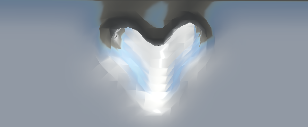
\includegraphics[width=3.4in]{figures/voxelize-fail.png}
\caption{After repeated pipe creation, the mesh containing these pipes, which were not originally intersecting, accumulated sufficient error to open the pipes into each other.}
\label{fig:voxelize}
\end{figure}


\subsection{Fabrication Techniques}

The physical fabrication process used by different machines gives rise to differing strategies for avoiding support material or easing its removal.  The two machines we used to create our example objects were the Objet Connex 260 and the Makerbot Replicator 2.

The Objet is an inkjet-based 3D printer which jets drops of polymer in very fine layers, curing each layer with an ultraviolet lamp.  It offers a wide range of material types, including clear/opaque, flexible/hard, and black/white.  Additionally, it permits the mixing of two different materials in a single print: a mixed material could include 70\% flexible and 30\% hard, for example, to be firm but somewhat flexible.  The flexible materials can be inflated when they are thin: they elongate 200\% before breaking.  We have found $.05$ inches to be a good thickness for inflatable materials.  Although this machine has many extraordinary capabilities, it unfortunately cannot print overhangs of greater than $14^{\circ}$ without support material.  Due to this, support avoidance is difficult; our main tactic for removing support material has been to make the \emph{openings} to pipes as large as possible.  This allows us to flush the material most easily.  The support structure used by this machine is a loose matrix of material that can be removed by hand from the surface, blasted out with a water jet from cavities, or dissolved in lye (the enclosing model material does not dissolve).

The Makerbot Replicator 2 is a fused-deposition modeling (FDM) printer, in which we use exclusively Polylactic Acid (PLA) bioplastics.  More material properties are being explored in PLA: there are now transparent and flexible materials.  They cannot be blended like those in the Objet.  The Makerbot has a fairly coarse resolution compared to the Objet, however it permits overhangs up to $45^{\circ}$ without support and also allows bridging (short spans of material that bridge the gap between two structures with no support underneath).  Although spheres and sideways cylinders have a $>45^{\circ}$ overhang in some places, they are also printable without support.  Due to the FDM process it can even recover from greater overhangs and longer bridges, as the material builds up and can reorganize into a structure \valkyrie{how do I say this?  do I need a photo?  print recovery is pretty awesome-looking.}.  The support used by the Makerbot is made of the same material as the model itself, just printed in a different pattern and attached over as small a surface area as possible to ease removal.  Support inside of a pipe may require pliers, or be infeasible to remove dependent upon geometry.  Meshmixer has a built-in tool for minimizing support for prints; it re-orients the part to keep as much surface area as possible within the 45 degree constraint.  In future work we would like to explore a tool in which a user can select surfaces to prioritize support avoidance for.

Assembly is easiest on both machines when the model does not require support material.  For especially complex geometries, models can be ``cut up'' \bjoern{This negates some of the benefits compared to other manufacturing techniques.} into assembleable pieces that evade support requirements or ease material removal.  We believe that an automatic tool for this task would be highly beneficial, however it is outside the scope of this work.